
\documentclass[10pt]{article}% uses letterpaper by default

%---------- Uncomment one of them ------------------------------
\usepackage[includeheadfoot, top=1in, bottom=1in, hmargin=1in]{geometry}

% \usepackage[a5paper, landscape, twocolumn, twoside,
%    left=2cm, hmarginratio=2:1, includemp, marginparwidth=43pt, 
%    bottom=1cm, foot=.7cm, includefoot, textheight=11cm, heightrounded,
%    columnsep=1cm, dvips,  verbose]{geometry}
%---------------------------------------------------------------
\usepackage{fancyhdr}
\usepackage{verbatim}
\usepackage{url}
\usepackage{cancel}
\usepackage{bbding}
\pagestyle{fancy}
\usepackage{amsmath}
\usepackage{graphicx}
\usepackage{setspace}
\usepackage{amssymb}
\usepackage{epstopdf}
\usepackage{wasysym}
%\doublespacing
\singlespacing
%\onehalfspacing
%\newcommand{\exercisename}{}



\newcommand{\degrees}{\ensuremath{^\circ}}
\newcommand{\arcmin}{\ensuremath{'}}
\newcommand{\arcsec}{\ensuremath{"}}
\newcommand{\hours}{\ensuremath{^\mathrm{h}}}
\newcommand{\minutes}{\ensuremath{^\mathrm{m}}}
\newcommand{\seconds}{\ensuremath{^\mathrm{s}}}

\newcommand{\s}[0]{\phantom{i}} %sets up \s command
\newcommand{\m}[0]{\phantom{abcde}} %sets up \m command
\providecommand{\e}[1]{\ensuremath{\times 10^{#1}}} %sets up \e command



\lhead{CCDs and Photometry}
\chead{}
\rhead{}
\lfoot{Spring Observing Lab 02}
\cfoot{\thepage}
\rfoot{}

\begin{document}

\begin{center}
{\huge CCDs and Photometry}\\ 
\end{center}

\section{Introduction}
\indent\indent The invention of the Charge Coupled Device (CCD) has revolutionized photography. All digital cameras -- even the one in your cell phone -- utilize this technology to create digital images. The ability to control exposure time and instrument sensitivity has enabled precise measurements of the brightness of stars, galaxies, and other astronomical objects and has allowed astronomers to study the universe in great detail. In this lab we will first learn some basics about CCD technology and its applications to astronomy, then we will use a digital camera to take images of stars which we will use in the next lab to measure properties about them.

\section{The Basics of the CCD}
\indent\indent To understand the basics of how a CCD works, we will work through an interactive tutorial found here: \url{http://bit.ly/CCDLab}. As you progress through the tutorial, answer any questions in your lab notebook. 

\section{More on Filters}

Color vision is the result of millions of microscopic filters in our eyes known as cone cells. There are three different types of cone cells corresponding to three different colors of light. These are blue, green and red corresponding to short, medium and long wavelengths (shown in Figure \ref{cones.fig}). The higher the ``transmission'' on the y-axis the more light that cone receives at that wavelength. Your brain assesses how much light is coming from each type of cone and translates this into the colors we see. If you don't have that cone, then your brain doesn't have information about those wavelengths --  this is what leads to color blindness.

\begin{figure}[h]
\center
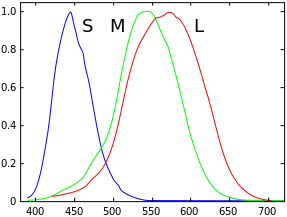
\includegraphics[scale=0.6]{cones.png}
\caption{This plot shows the \textbf{filter response} curves of the three different cones of your eyes. The x-axis is wavelength of light. The y-axis is ``transmission.''  A transmission of 1 means all light of that wavelength makes it through the filter and that cone is most sensitive. A transmission of 0 means no light of that wavelength is perceived by that cone.  \label{cones.fig}}
\end{figure}

A common question about astronomical images is whether the objects actually look the way they do in an image. The answer is not a simple yes or no, and depends on the instrument and filters used to take the image. \textit{Optical filters} can often mimic the filter response of the human eye, so a color image made with three optical filters will look like true color if the object is bright enough. \textbf{If we took an image of a galaxy using three filters that identically match the response of the cone cells in the human eye and compared this to looking at the object through a telescope, would it look the same? If not, what about the two views would be different?}

\section{Exposure Time}
A crucial aspect of photography is the ability to set the exposure time when taking an image. Your eye processes the light it sees almost instantaneously, which is useful in a bright, always-changing world. For imaging distant or faint objects, we need to be able to collect light for longer periods of time.

The following calculations demonstrate the advantage of longer exposure times. 

\subsection{Limits of the Human Eye}
Scientists have found that in order for our brain to register a detection of light, we must receive at least \textbf{5 photons} within approximate \textbf{100ms}.  In general, the width of the human pupil is about 10mm and a typical visible photon has a wavelength of 510nm. 

The flux your eye receives is the total photon energy per unit time per collection area of your eye.  \textbf{Combine the following equations to calculate the flux-limit of the human eye.} (Keep everything in SI units.)

\begin{equation}
\mathrm{Flux_{limit}} = \frac{\mathrm{total} \ E}{\mathrm{Area}*t}
\qquad
E_{\mathrm{photon}} = \frac{hc}{\lambda}
\qquad
\mathrm{Area}_{\mathrm{circle}} = \pi r^2
\end{equation}

Useful constants:
\begin{equation}
h = 6.626 \times 10^{-34} J \\ s
\qquad
c = 3.0 \times 10^8 m/s
\end{equation}

Now that we know the limits of our eye, \textbf{how far away could the Sun be and we still be able to see it?} Rearranging these equations gives the answer:
\begin{equation}
F = \frac{L}{4\pi d^2}
\qquad
L_{sun} = 3.839 \times 10^{26} \  \mathrm{W}
\qquad
1 \mathrm{pc} = 3.09 \times 10^{16} m
\end{equation}

The Galactic center is at a distance of 8kpc or 8000pc.  Be careful of your units!

\section{Imaging Stars}
For the next section of the lab, we will be going up to the roof to take images of stars using a camera mounted on one of the telescopes. In the next observing lab we will use the data collected by all lab sections to learn something about the internal properties of stars using just the color information we get from the filters in the camera.

\subsection{Choosing your targets}
Using planispheres from the previous observing lab, choose 10 stars that will be visible when we are on the roof. Make a table in your lab notebook like this:

\begin{center}
	\begin{tabular}{| p{3cm} | p{3cm} | p{5cm} |}
	\hline
	  \textbf{Name} & \textbf{Color} & \textbf{Filename} \\
	 \hline
	 \hline
	  Star A &  &  \\
	  \hline
	  Star B &  &  \\
	  \hline
	  ... &  & \\
	  \hline
	\end{tabular}
\end{center}

\subsection{Visual classification}
Now we will go to the roof. Find each of your targets with your naked eye, a pair of binoculars, or a Dobsonian telescope (on the roof). Write down in your table whether each star looks white, blue, orange, red, etc. (in the color column). Now choose three stars that have \emph{different} colors -- for example, I could choose one blue star, one orange star, and one white star. Put a check mark next to the names of these three targets. Your table should now look something like this:

\begin{center}
	\begin{tabular}{| p{3cm} | p{3cm} | p{5cm} |}
	\hline
	  \textbf{Name} & \textbf{Color} & \textbf{Filename} \\
	 \hline
	 \hline
	  Star A &  Blue &  \\
	  \hline
	  Star B \Checkmark & Blue &  \\
	  \hline
	  Star C \Checkmark & Red &  \\
	  \hline
	  ... &  & \\
	  \hline
	\end{tabular}
\end{center}

\subsection{Taking images}
We will now use a digital camera mounted on a telescope in the ``Little Dome'' to take images of your three selected targets. Follow the instructions of the TA, and \textbf{make sure to write down the image filename in the appropriate table row}! The procedure to take an image will be:

\begin{enumerate} 
	\item Use the telescope finder scope and hand paddle to center your target star in the viewfinder of the camera;
	\item xxx
\end{enumerate}

\end{document}


